\chapter{适应未知背景的可微分渲染方法}
\label{chap:method}

在将可微分渲染方法应用到3D人脸重建任务时,现有方法均未能充分利用可见性梯度。
而该梯度正是所有梯度中的主要分量,对模型与照片的精确对齐有着重要作用。
通常来说,计算正确的可见性梯度需要同时具有前景和背景的模型,而在自然环境照片中,由于背景多样,很难得到显式的背景模型。
本章主要针对该问题,提出一种适应未知背景的可微分渲染方法,能够利用可见性梯度来优化模型与照片的对齐。

\section{问题定义}

可微分渲染旨在从参数化的3D模型,如三角形面片,纹理贴图等,渲染得到2D图片,同时计算该渲染结果关于其输入参数的梯度。
然后可以优化渲染结果与照片间的误差,以期利用基于梯度的方法优化输入参数,从而改善渲染效果,使之更加接近现实。
其在3D人脸重建的相关任务中已有较广泛的应用。

然而现有方法存在一些不足:
现有可微分渲染技术大多是对整张图片估计梯度,即不区分前景和背景部分。
但是,在基于自然环境照片的人脸重建任务中,我们通常只有前景(即人脸)的3D模型,而没有背景的模型。
此时,现有方法选择忽略模型间相互遮挡产生的可见性梯度,而这会造成模型与照片的对齐不准确,如图\ref{fig:problem_a}所示。
另一方面,若对背景进行很粗糙的建模,例如假设为全黑,则错误的梯度会导致模型无法正确收敛,如图\ref{fig:problem_b}所示。

\begin{figure}
\centering
\begin{subfigure}[t]{0.45\textwidth}
    \centering
    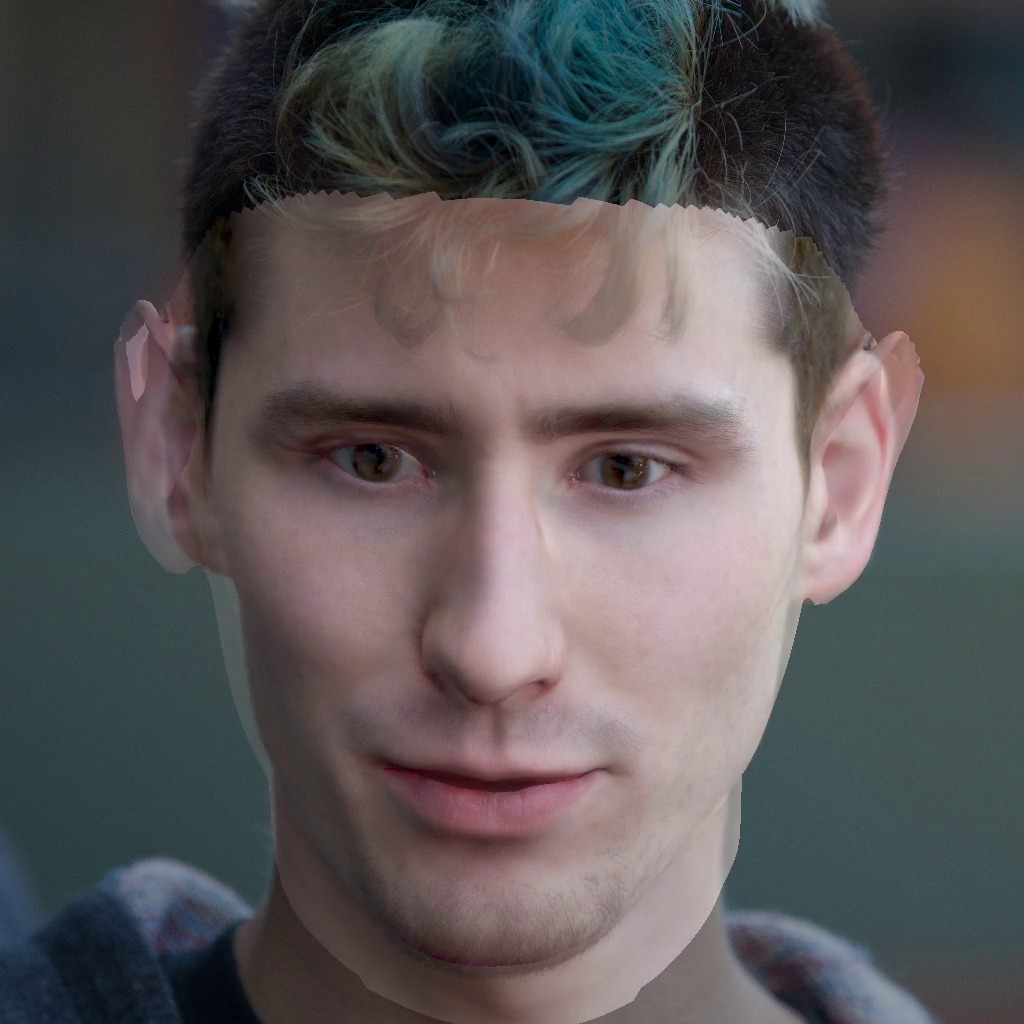
\includegraphics[width=\textwidth]{figures/black-bg_no-aa}
    \caption{忽略可见性梯度,模型与照片未准确对齐}
    \label{fig:problem_a}
\end{subfigure}
\begin{subfigure}[t]{0.45\textwidth}
    \centering
    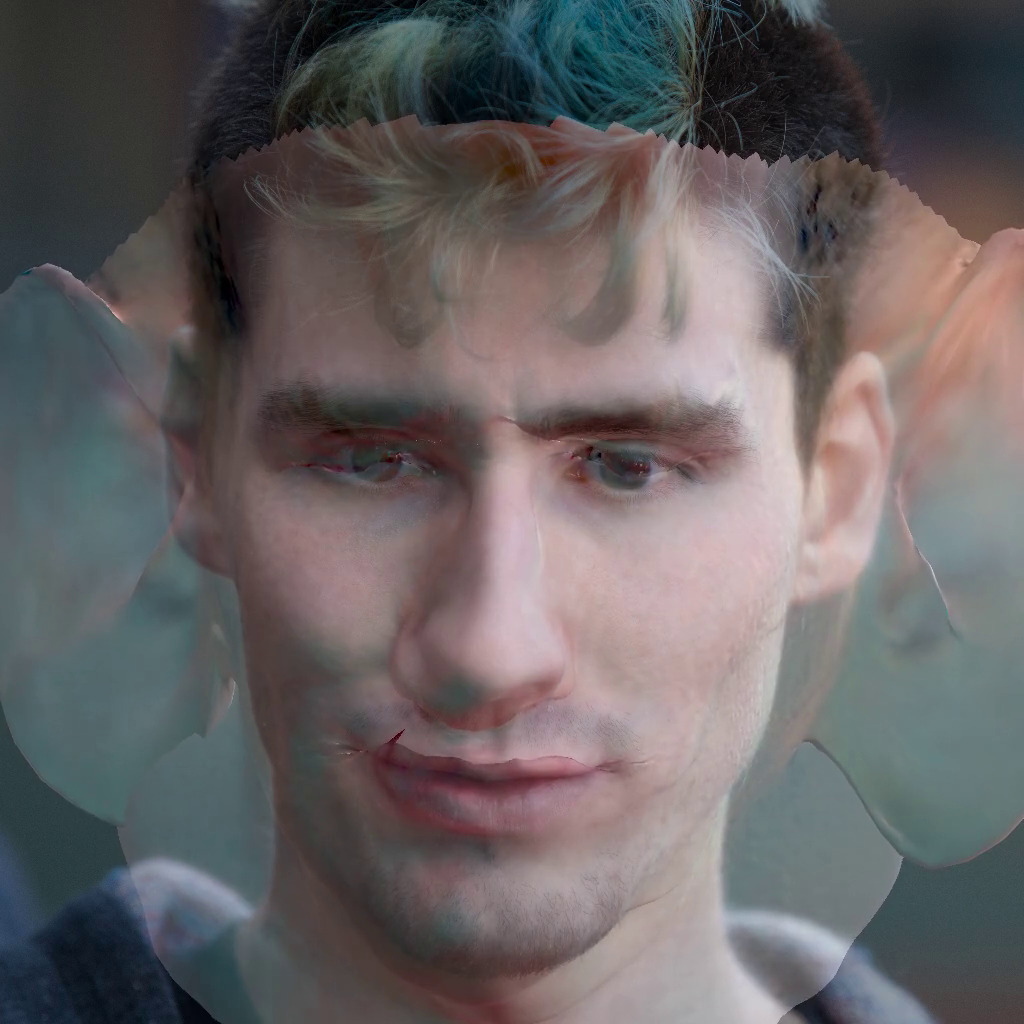
\includegraphics[width=\textwidth]{figures/black-bg}
    \caption{使用全黑代替背景模型,可见性梯度错误}
    \label{fig:problem_b}
\end{subfigure}
\caption[未知背景条件下可微分渲染优化结果]{
    未知背景条件下可微分渲染优化结果。
    示意图为目标照片和渲染结果以1:1 alpha混合后,再进行gammar校正得到。
}
\end{figure}

为绕过上述问题,现有方法通常:
使用多目立体等其他手段事先确定高精度的人脸几何形状,并在逆渲染优化过程中使几何形状保持不变\citep{RiviereGBGB20};
忽略可见性梯度,使用2D人脸关键点\citep{deep3d}、图像分割\citep{nvdiffrec}结果等辅助监督信息来补足这部分缺失的梯度。
但是,如果能够直接利用可见性梯度,可大大简化算法的流程,同时也能避免在前序步骤中引入额外的误差。

本节将设计一个简单的玩具实验来更直观地说明上述问题。
如图\ref{fig:problem}所示,我们使用一个简单的白色平面作为前景模型,用其拟合一个白色青色对半分割的场景。
该模型的参数是其横向的平移量,用平面边缘与横坐标轴的交点$a_x$表示。
该平面的边缘稍微倾斜,以突出可见性梯度的变化。
该平面的着色不受参数影响,始终固定为白色。
该例子中使用的损失函数为L1误差,即:
\begin{equation}
\mathcal{L} = \left\| \hat{\mathcal{I}} - \mathcal{I} \right\|_1
\text{。}
\end{equation}

\begin{figure}
\centering
\import{build/figures}{problem.pgf}
\caption[在未知背景时计算可见性梯度困难]{
    在未知背景时计算可见性梯度困难。
    拟合目标和渲染结果左侧白色为前景,右侧为背景。
    前景模型为以红线为边界的白色平面。
    横坐标为前景模型的平移量。
    a)离散采样,不计算可见性梯度;
    b)使用不准确的黑色背景模型计算可见性梯度,模型无法收敛到期望位置;
    c)理想情况下,在完全已知背景时的可见性梯度,模型能准确收敛至梯度为0的点。
}
\label{fig:problem}
\end{figure}

其中,a)为离散采样的方式,也是目前大多人脸重建中使用的方法。
其渲染流程为:在每个像素的中点处采样,若其位于前景模型的覆盖范围内,则渲染为白色,否则渲染为背景。
由于采样过程是离散的,且$a_x$的改变并不会影响采样的模式,因此,渲染结果$\hat{\mathcal{I}}$关于$a_x$的梯度为0,其损失函数为阶梯函数。
即该损失函数完全无法以基于梯度的方式指导模型拟合。

另一方面,在没有准确背景模型的前提向,可见性梯度则难以被利用。
例如,在b)中,假设我们并不知道该场景的背景,因此直接假设其为全黑。
但在本例中这个假设显然是不准确的。
在此前提下,从图中可以观察到其损失函数呈递减的趋势,并未在期望的位置上形成极值。
因此,该梯度也无法引导模型收敛到期望的位置。

作为参考,c)展示了理想中,完全已知背景的情况下,可见性梯度的作用。
从图中可见,其损失函数在期望的位置上有一个明显的极值,且其周围的梯度将能很好地指导优化器,使模型收敛到该位置。

然而,在实际人脸重建的任务中,特别是从自然环境照片的重建中,背景可能是很复杂且难以建模的。
本章将探讨如何在这种情况下,如何利用可见性梯度以指导前景模型与目标照片对齐。

\section{本文方法}

收缩\&扩展约束(创新点)

\section{实验结果}

\section{讨论}

L1损失函数的必要性
